\documentclass[a4paper,twocolumn]{article}
\usepackage{listings}
\usepackage{amsmath}
\usepackage{tikz}
\usepackage{sectsty}
\title{Domination is not a Tree \\
\Large{Towards More Precise Domination Relations}}
\date{Jan 25, 2024}
\author{George Stelle \; Tarun Prabhu \; Pat McCormick \\ Los Alamos National Laboratory}

\lstdefinestyle{mystyle}{
  basicstyle=\ttfamily
}
\lstset{style=mystyle}
\sectionfont{\fontsize{12}{15}\selectfont}

\begin{document}
\maketitle

In LLVM and other modern compilers, single static assignment (SSA) is a crucial
theory for internal representations, enabling optimizations in the presence of
imperative code. A fundamental function of SSA is calculating and using
domination relations to determine where immutable variables can be referenced.
Dominator trees have historically been a good approximation of the dominator
relation and efficiently computable. Unfortunately, there are programs for
which the dominator tree fails to capture precise domination relations,
preventing optimizations. In this work, we will give examples of these kinds of
programs, and show how removing the restriction to trees enables more precise
domination relations, therefore enabling more optimization. We discuss how one
can use properties of SSA to implement a more general domination relation using
a small set of trees corresponding to shared branches, which we call a
dominator \emph{grove}. 

\section*{Theoretical Motivation}
Recall the definition of domination in the context of programs: a node $a$
dominates a node $b$ if every \emph{valid} path from the entry block to $b$ goes
through $a$. Note that we specify valid paths explicitly, as historically
domination has focused on any path through the control flow graph (CFG).
Because we care about domination in \emph{programs}, we need to reason about
valid paths beyond just the CFG. 

To understand non-tree domination relations, consider the following simple
example: 
\begin{minipage}{\linewidth}
\begin{lstlisting}[language=C]
void f(bool c, int x){
  int y = 0;         \\ entry
  if(c) y = pre(x);  \\ pre
  body(x);           \\ body	
  if(c) post(y);     \\ post
}
\end{lstlisting}
\end{minipage}
Note that there are two valid paths through the program: one which calls
\texttt{pre} and \texttt{post} and one which doesn't. Therefore, by the
definition of domination, the call to \texttt{post} is dominated by the call to
\texttt{pre}. Representing the domination relations graphically gives: 
\begin{center}
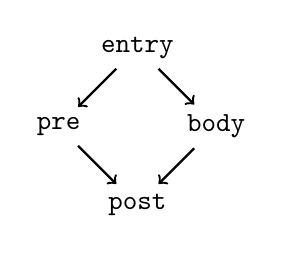
\begin{tikzpicture}[->, line width=0.3mm]
\node(entry) at (2,3) {\texttt{entry}};
\node(a) at (1,2) {\texttt{pre}};
\node(b) at (3,2) {\texttt{body}};
\node(c) at (2,1) {\texttt{post}};
\path
(entry) edge (a)
(entry) edge (b)
(a) edge (c)
(b) edge (c);
\end{tikzpicture}
\end{center} 

\section*{Implementation}
The crucial property that lets us refine the notion of valid paths and
therefore refine the domination relation is that whenever there are multiple
conditional branches that share a static condition variable, we can construct
two distinct dominator trees that correspond to case analysis on the value of
the shared condition variable. If a domination relation holds for both
dominator trees, then it holds in the general case. We call this structure a
dominator \emph{grove}, as it contains a small set of trees. Because of this 
dependence on condition variables, one can view this approach as a class of 
\emph{context-sensitive} domination relations. This is in contrast to the
dominator tree, which is computed solely with knowledge of the CFG, and no
further context.

We present an initial implementation of the dominator grove approach in LLVM.
By modifying the existing implementation of incremental dominator tree updates,
we show how one can extend the implementation of dominator trees to implement
dominator groves in a way that requires only a relatively small change to the
codebase. 

While the implementation successfully computes more precise domination
relations, there is a problem: existing code doesn't just query domination
relations: it \emph{assumes dominator tree structure}. These assumptions are
violated by the more precise domination relations, causing compiler bugs. We
discuss some of the challenges in removing these assumptions from LLVM, and
hope to get feedback from the community on the cost of addressing these
assumptions.

\section*{Empirical Motivation}
In the above example we've shown the existence of programs with non-tree
domination relations, but a natural question is how often these kinds of
programs occur in the wild. To measure this, we run the implementation
described above on \texttt{llvm-test-suite}. We discover that out of the
$\sim55$ million calls to \texttt{dominates}, $\sim1.9$ million calls are made
more precise by the dominator grove, or $\sim3.5\%$. This shows that there are
a non-trivial number of non-tree domination relations in real world code. We
look forward to discussing a further breakdown of the data with the community.

\section*{Concurrency}
In addition to improving optimizations for sequential programs, we argue that 
removing the tree constraints from domination relations is necessary to build a
concurrent SSA theory. To be able to run two pieces of code concurrently, then
wait for them to finish, we need to be able to represent that neither dominate
each other, but both dominate the join point. We look forward to discussing
with the community further how SSA and LLVM can be extended with concurrent
semantics, and why the dominator tree constraint must be relaxed to take full
advantage of optimizations in the presence of concurrency.

\end{document}
